\documentclass{article}

\usepackage{graphicx}
\usepackage{amsmath}
\usepackage{float}

\title{PA5: Sorting}
\author{Kevin Lei}
\date{April 19, 2024}

\begin{document}

\maketitle

\section{Introduction}
The purpose of this programming assignment is to implement four different sorting algorithms: bubble sort, heap sort, merge sort, and quick sort.
In this report we will discuss the theoretical performance of each algorithm, devise an experimental setup to test the performance of each algorithm, and present the results of the experiment.

\section{Theoretical Analysis}
In this section we will analyze the theoretical performance of each sorting algorithm.

\subsection{Bubble Sort}
The bubble sort algorithm works by iterating through the array and swapping adjacent elements if they are in the wrong order.
This process is repeated until the array is sorted.
The average and worst case time complexity of bubble sort is $O(n^2)$, where $n$ is size of the array, since the number of inner loops is proportional to the array size, and the number of comparisons in each inner loop is also proportional to the array size.
The best case time complexity of bubble sort is $O(n)$, which occurs when the array is already sorted.
Bubble sort is known for its simplicity and poor performance compared to other sorting algorithms, due to its quadratic time complexity.

\subsection{Heap Sort}
The heap sort algorithm works by first building a max heap from the array, then repeatedly extracting the maximum element from the heap and placing it at the end of the array.
The average, worst, and best case time complexity of heap sort is $O(n \log n)$, where $n$ is the size of the array.
This is due to the fact that there are $n$ elements to insert into the heap, and each insertion takes $O(\log n)$ time.
After the heap is built, creating the sorted array requires $n$ extractions, each of which takes $O(\log n)$ time.
Therefore, the total time complexity is $O(n \log n)$.

\subsection{Merge Sort}
The merge sort algorithm works by first recursively dividing the array into halves until each subarray becomes an empty array or a singleton array.
Then, the subarrays are merged back together in sorted order.
The best case time complexity of merge sort is $O(n)$, which is when the array is already sorted.
The average and worst case time complexity of merge sort is $O(n \log n)$, where $n$ is the size of the array.
The time complexity can be derived as follows:
\begin{align*}
    T(1) &= 1 \\
    T(n) &= 2T(n/2) + 2
\end{align*}
\begin{align}
    T(n) = 2T(n/2) + 2n &\longrightarrow T(n) = 2(2T(n/2^2 + n) + 2n \\
    T(n) = 2^2T(n/2^2) + 4n &\longrightarrow T(n) = 2^2(2T(n/2^3) + n/2) + 4n \\
    T(n) = 2^3T(n/2^3) + 6n &\longrightarrow T(n) = 2^3(2T(n/2^4) + n/2^2) + 6n \\
    \vdots \nonumber \\
    T(n) &= 2^kT(n/2^k) + 2kn \nonumber \\
    \text{Solving the base case: }& n/2^k = 1 \rightarrow n = 2^k \rightarrow k = \log n \nonumber \\
    T(n) &= 2n \log{n} + n \in O(n \log n) \nonumber
\end{align}

\subsection{Quick Sort}
The quick sort algorithm works similarly to merge sort, but instead of sorting by merging sorted arrays, quick sort works by partitioning the array into two subarrays around a pivot element.
The worst case time complexity of quick sort is $O(n^2)$, which occurs when the pivot element is the smallest or largest element in the array, resulting in an unbalanced partition.
However, in the average case, quick sort has a time complexity of $O(n \log n)$, which is the same as merge sort.
It is worth noting that although quick sort has the same time complexity as merge sort, quick sort is generally faster in practice due to its lower constant factors.

\section{Experimental Setup}
To test the performance of the sorting algorithms, random arrays of integers were generated and sorted using each algorithm.
The sizes of the arrays include 10, 100, 1000, 10000, 100000, and 1000000 elements.
One trial was conducted for each array size.

\section{Experimental Results}
The results of the experiment are shown in the following graphs.

\begin{figure}[H]
    \centering
    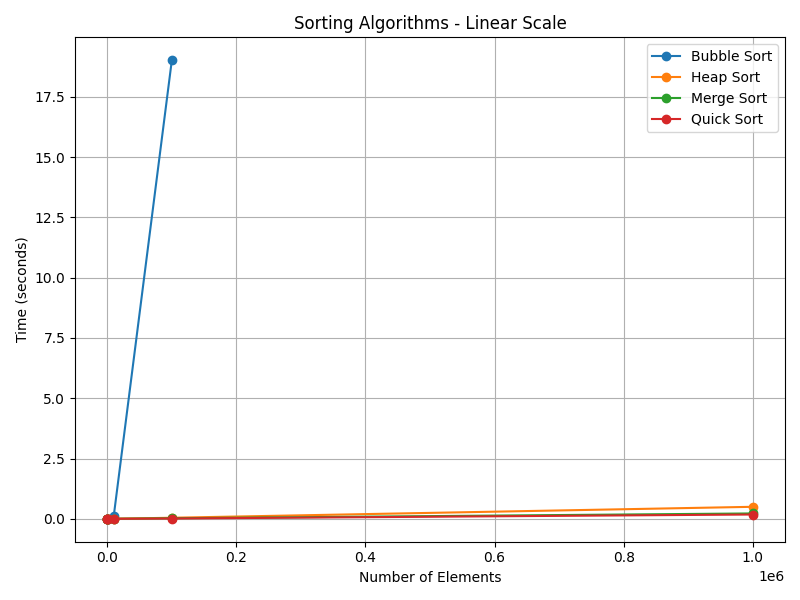
\includegraphics[width=0.9\textwidth]{../plotting/linear.png}
    \caption{Performance of sorting algorithms using a linear scale.}
\end{figure}

\begin{figure}[H]
    \centering
    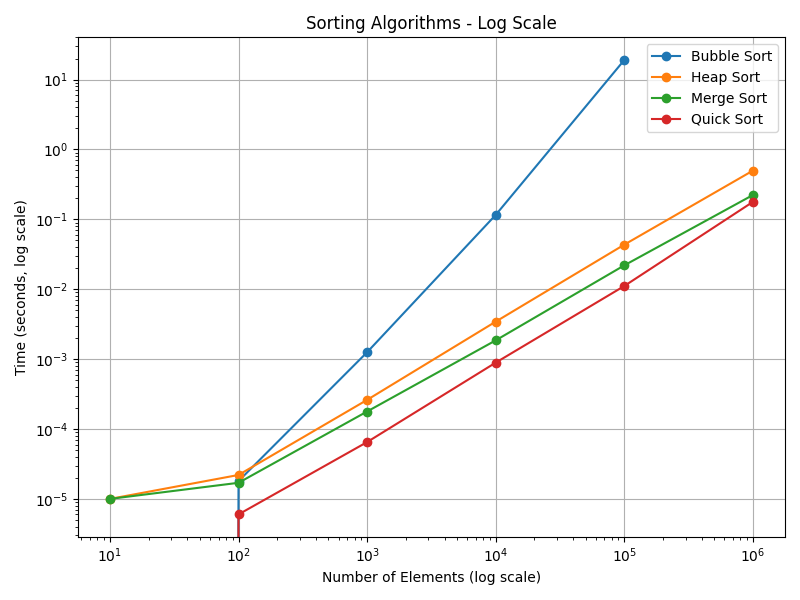
\includegraphics[width=0.9\textwidth]{../plotting/log.png}
    \caption{Performance of sorting algorithms using a logarithmic scale.}
\end{figure}

The most immediate result we can observe from these graphs is that bubble sort is indeed by far the slowest sorting algorithm.
It's time complexity of $O(n^2)$ is clearly reflected in the graphs, and almost single-handedly necessitates the use of logarithmic scales to properly visualize the performance of the other sorting algorithms.
Even then, we exclude the last input size of 1000000 elements for clarity.

Aside from the poor performance of bubble sort, the other sorting algorithms perform as expected, all within the bound of $O(n \log n)$.
Within these three better algorithms, we observe heap sort to be the slowest across all input sizes.
This could be due to the large amount of constant factors in heap sort, since it requires multiple passes through the array to build the heap and extract the maximum element.
Merge sort and quick sort perform very similarly, with quick sort being slightly faster in our tests. 
We also notice that the difference between merge sort and quick sort becomes less pronounced as the input size increases, with quick sort being almost overtaken by merge sort at the largest input size of 1000000 elements.
This could be due to the fact that quick sort has a worse worst case time complexity of $O(n^2)$, which could be more likely to occur with larger input sizes.

\end{document}